\begin{frame}{Hamiltonian, and Basis, and Rabi Oscillations}



\begin{tcolorbox}[title=Hamiltonian in Background Matter Basis]
    \begin{equation*}
    \mathbf {H} = \frac{1}{2}\left( - \omega_{\mathrm{m}} + {\color{red}\delta \lambda(x)} \cos 2\theta_{\mathrm{m}} \right) \sigma_3 - \frac{  {\color{red}\delta \lambda(x)}  }{2} \sin 2\theta_{\mathrm{m}} \sigma_1.
\end{equation*}
\end{tcolorbox}


Matter profile
\begin{equation*}
    \lambda(x) = \lambda_0 + {\color{red}A \cos (k x)},
\end{equation*}


\begin{equation*}
    \mathbf {H} = \frac{1}{2}\left( - \omega_{\mathrm{m}} +  \cos 2\theta_{\mathrm{m}}{\color{red}A\cos(kx)} \right) \sigma_3 - \frac{  \sin 2\theta_{\mathrm{m} }  }{2}{\color{red}A \cos(kx)}  \sigma_1.
\end{equation*}





\end{frame}


\begin{frame}{Stimulated Neutrino Oscillations}


\only<1-1>{
% Matter profile
\begin{tcolorbox}[title=Matter Profile]
\begin{equation*}
    \lambda(x)  = \lambda_0 + {\color{red}\delta\lambda(x)}
\end{equation*}
\end{tcolorbox}


% Basis


\begin{tcolorbox}[title=Basis]

Background matter basis: Hamiltonian is diagonalized with only background matter profile $\lambda_0$,

\begin{equation*}
    \mathrm{H}_{\mathrm{background}} = -\frac{\omega_{\mathrm{m}}}{2} \boldsymbol{\sigma_3}.
\end{equation*}

\end{tcolorbox}


% Hamiltonian of with perturbation in matter profile, in background matter basis
\begin{tcolorbox}[title=Hamiltonian]

\begin{equation*}
    \mathbf H = \frac{1}{2}\left( - \omega_{\mathrm{m}} + {\color{red}\delta \lambda(x)} \cos 2\theta_{\mathrm{m}} \right) \boldsymbol{\sigma_3} - \frac{{\color{red}\delta \lambda(x) } }{2} \sin \theta_{\mathrm{m}} \boldsymbol{\sigma_1}.
\end{equation*}


\end{tcolorbox}

}

\only<2-2>{

% \begin{tcolorbox}
% Kneller, J. P., McLaughlin, G. C., \& Patton, K. M. (2013). J. Phys. G: Nucl. Part. Phys. {\bf{40}} (2013) 055002.
% \end{tcolorbox}

\begin{tcolorbox}
P. Krastev and A. Smirnov (1989); J. Kneller et al (2013);\\ K. Patton et al (2014);
\end{tcolorbox}


\begin{figure}
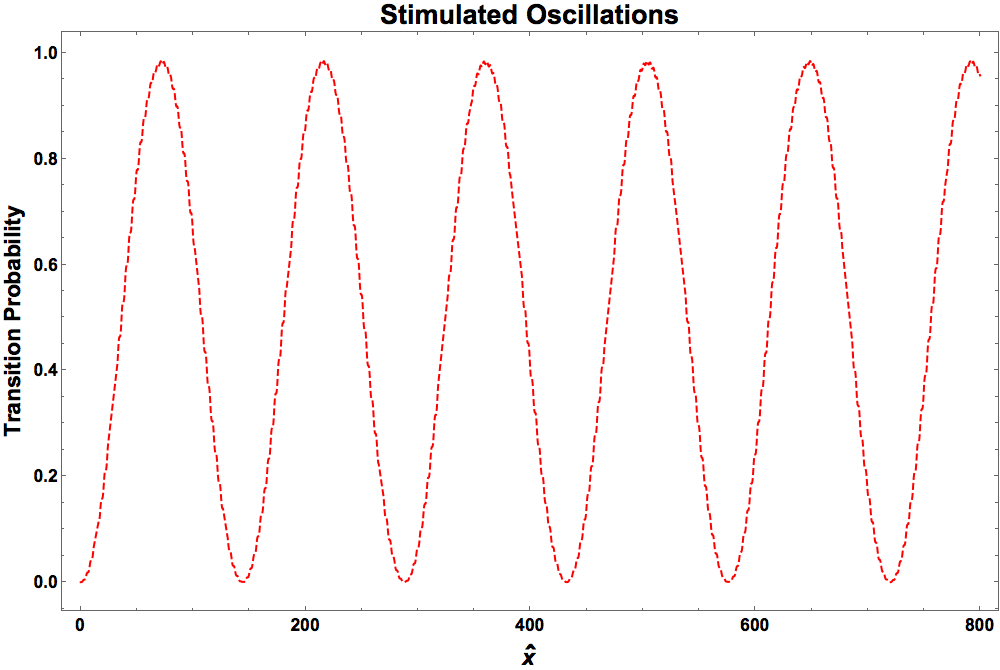
\includegraphics[width=0.8\textwidth]{assets/stimulated-oscillation-phenomenon.png}
%stimulated-neutrino-oscillations-kneller.png}
\caption*{Stimulated oscillations. $\lambda(x) = \lambda_0 +  A \sin (k x)$  with $\hat x = \omega_{\mathrm m} x $, $A=0.1\omega_{\mathrm m}$, $k=0.995\omega_{\mathrm m}$, $\theta_{\mathrm{m}}=\pi/6$}
\end{figure}


}





\end{frame}







%%%%%%%%%%%%%%%%%%%%%%%%%%%%%%
%%%% Neutrino Halo Problem






\begin{frame}{Neutrino Halo}

\only<1>{
\begin{figure}
   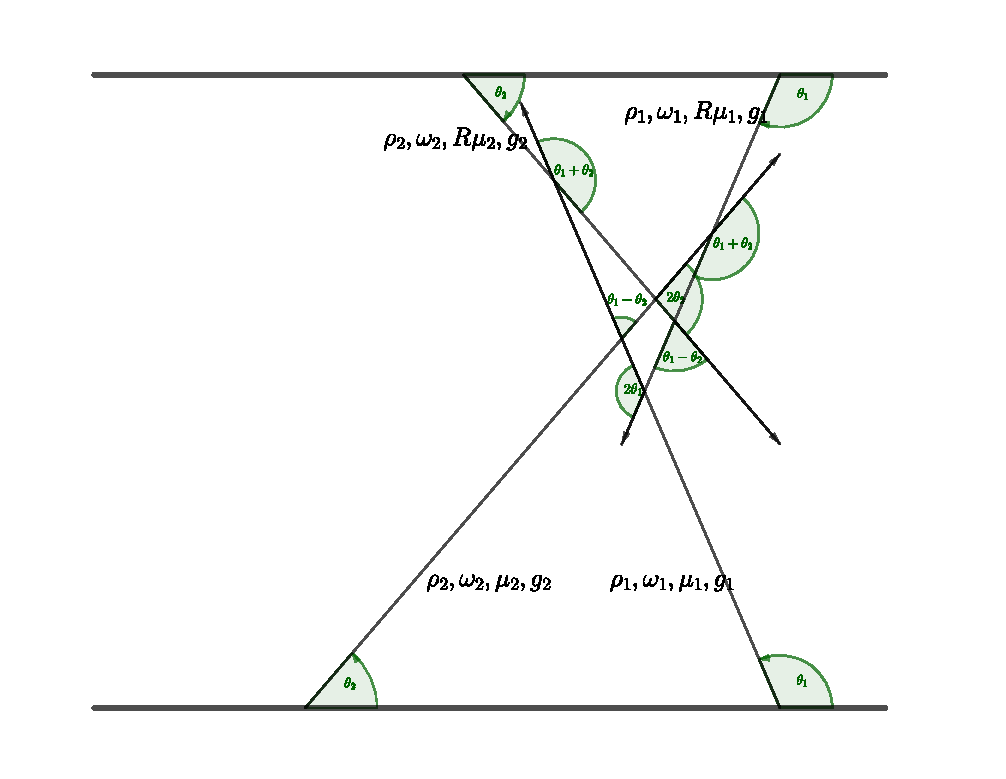
\includegraphics[width=\textwidth]{assets/halo-line-model}
\end{figure}
}

\only<2>{

\begin{columns}[T]
   \begin{column}{0.5\textwidth}
      Assumptions
      \begin{itemize}
         \item Neutrinos are translational symmetric on the emission line.
         \item Reflection obays Snell's law.
         \item Neutrinos are reflected on a fixed surface $z=L$.
         \item Neutrino reflections are translational symmetric.
      \end{itemize}

   \end{column}

   \begin{column}{0.5\textwidth}
      \begin{figure}
         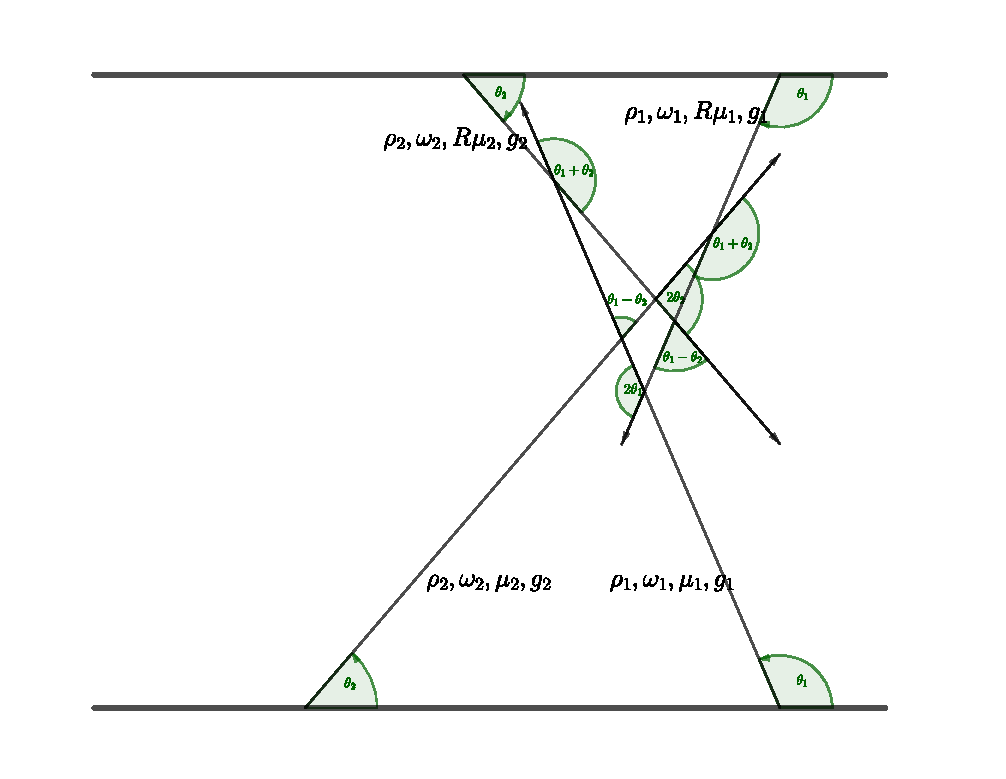
\includegraphics[width=\textwidth]{assets/halo-line-model}
      \end{figure}
   \end{column}
\end{columns}


}

\end{frame}

\subsection{Flavor Isospin Picture}

\begin{frame}{Flavor Isospin}


\begin{figure}
   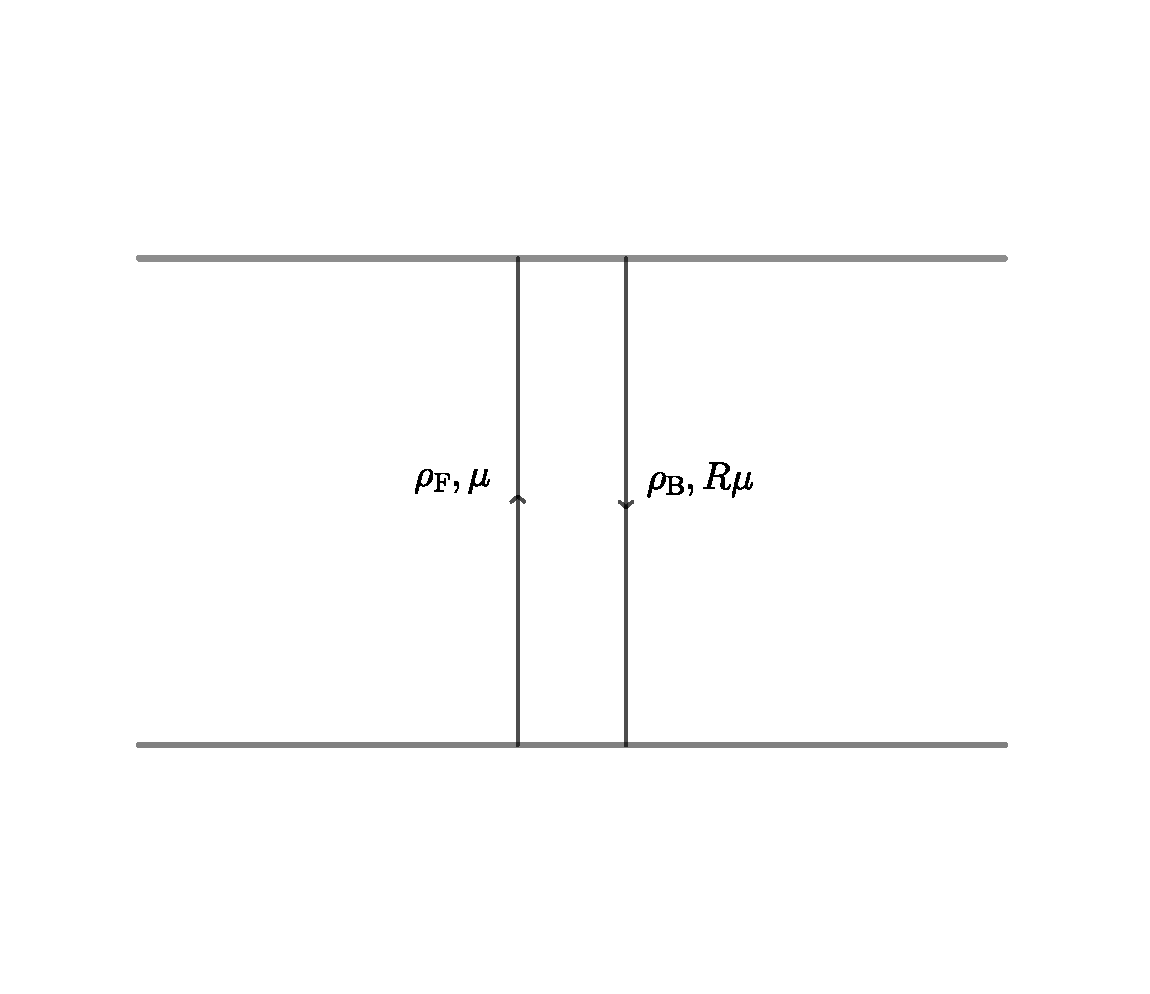
\includegraphics[width=\textwidth]{assets/halo-line-model-single-beam}
\end{figure}


\end{frame}



\begin{frame}{Relaxation Scheme}

\begin{tcolorbox}[title=Algorithm,standard jigsaw,
    opacityback=0]
   \begin{enumerate}
      \item Calculate forward beam using null backward beam;
      \item Calculate backward beam using forward beam calculated in step 1;
      \item Calculate forward beam using backward beam calculated in step 2;
      \item Repeat 2 and 3 until the beams reach equilibrium.
   \end{enumerate}
\end{tcolorbox}




\end{frame}




\begin{frame}{Numerical Method}

\begin{tcolorbox}
\begin{figure}
   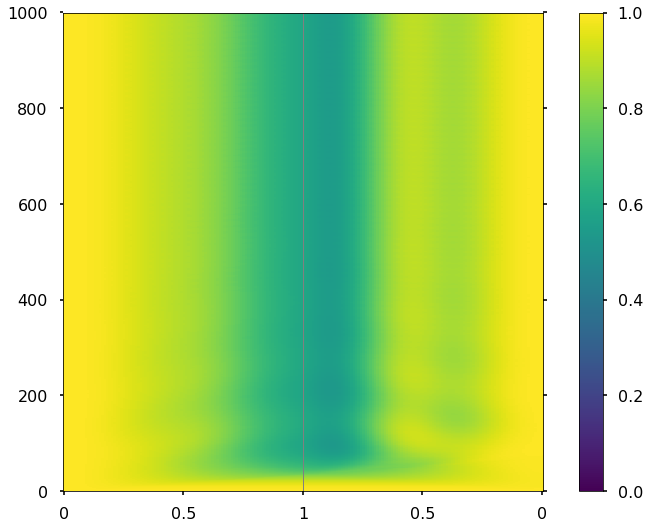
\includegraphics[width=0.9\textwidth]{assets/relax-color}
   \caption*{\color{black}Horizontal axis is the location of neutrinos; Vertical axis is the number of iteration steps; Color indicates the electron flavor probability.}
\end{figure}
\end{tcolorbox}

\end{frame}


\begin{frame}{Numerical Method}

\begin{tcolorbox}
   \begin{figure}
      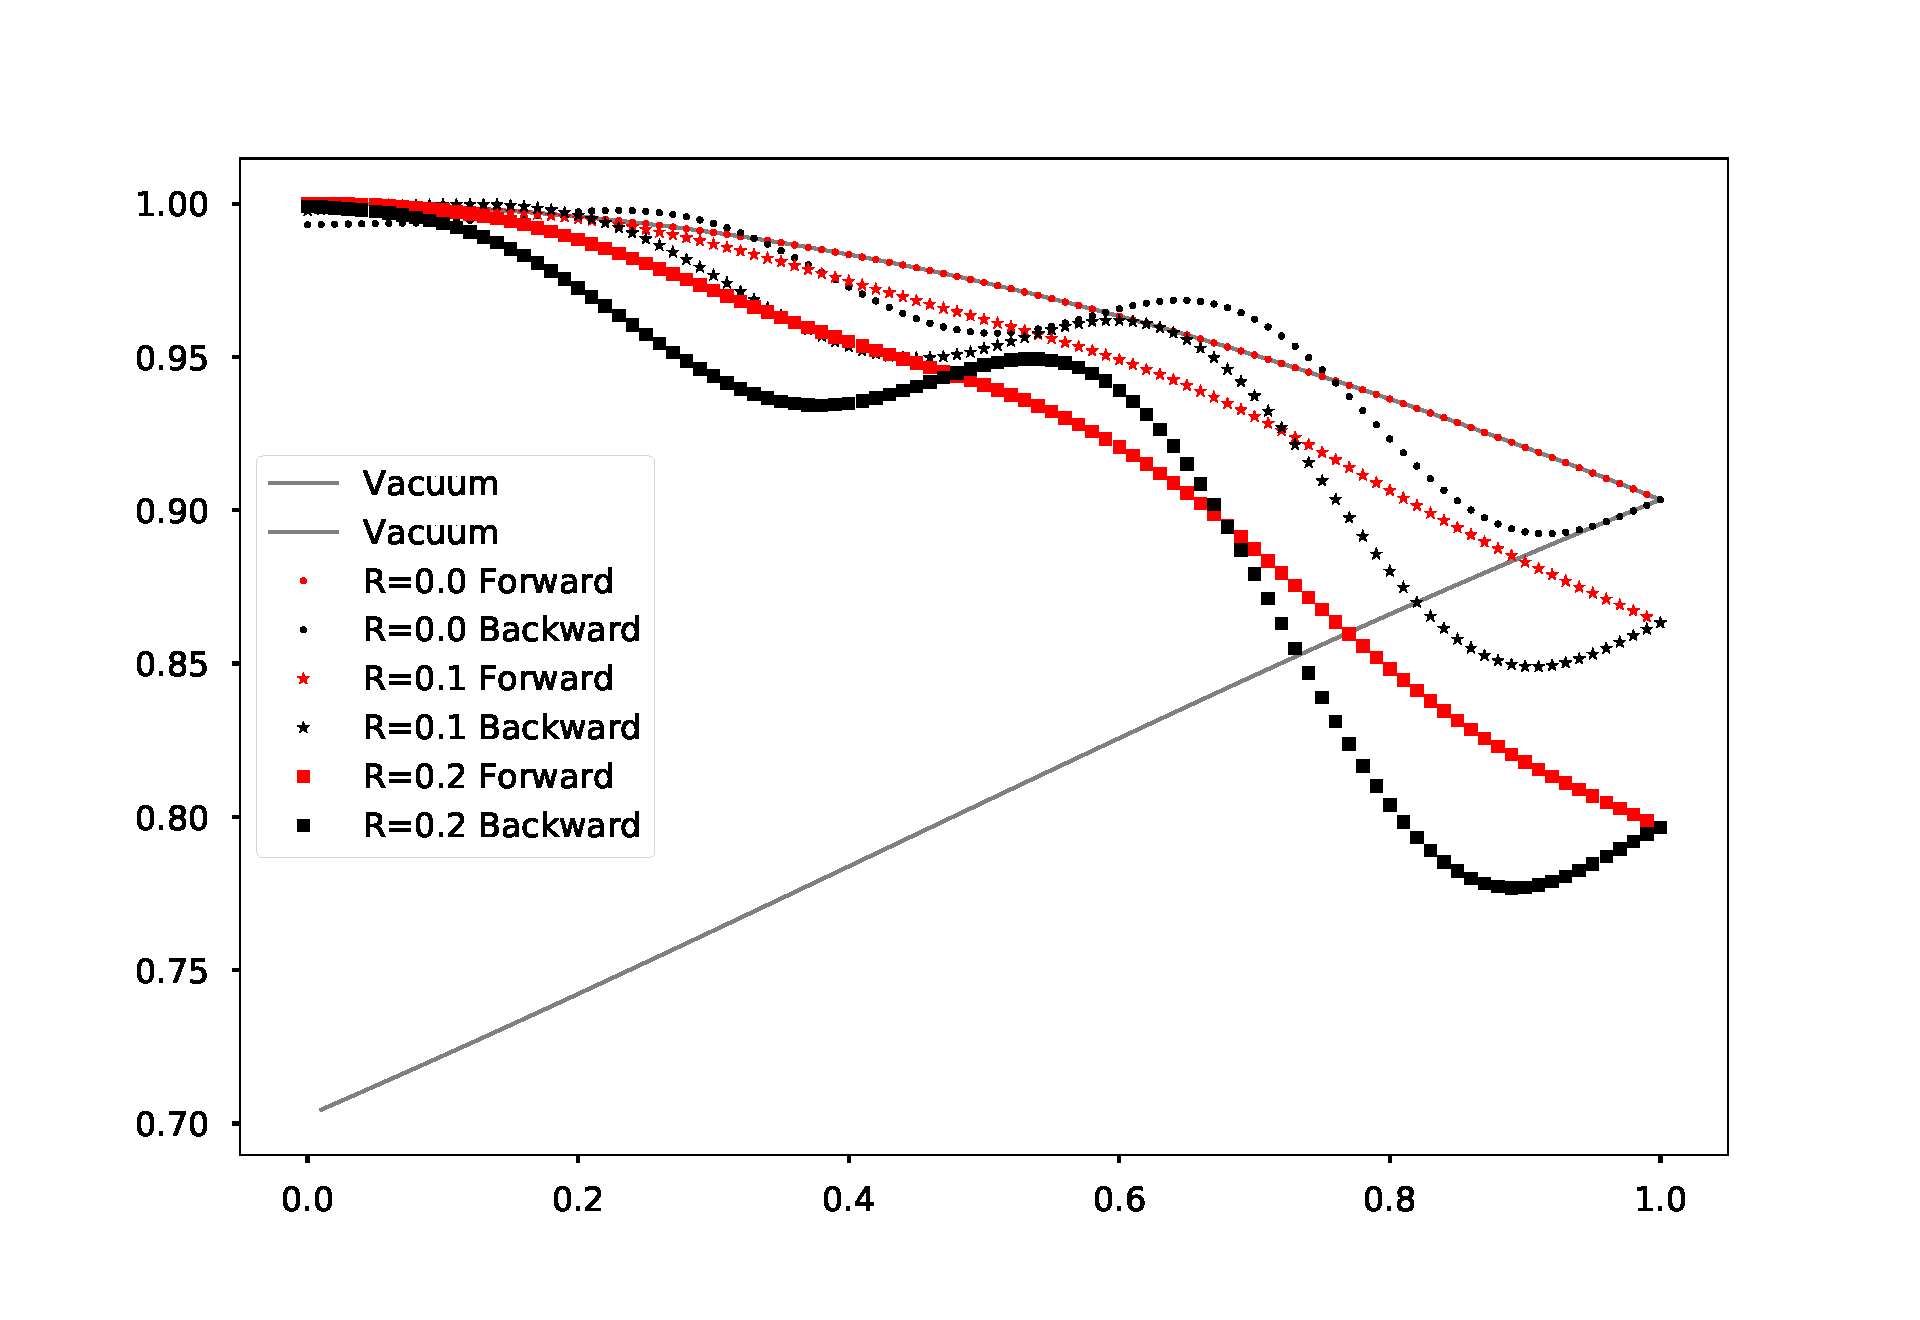
\includegraphics[width=\textwidth]{assets/halo-mu-4-r-multiple}
   \end{figure}
\end{tcolorbox}

\end{frame}

\begin{frame}{Linear Stability Analysis}

EoM

   \begin{align*}
    i \partial_t \vec s_F &= \mathbf s_F \times (\vec {H}_v +R \mu \vec s_B) \\
      i\partial_t \vec s_B &= \vec s_B \times (- \vec H_v - \mu \vec s_F) .
   \end{align*}

Compare with bipolar

\begin{align*}
    i\partial_t \vec s &= \mathbf s \times ( \eta \vec H_v + \alpha \mu \bar{\vec s} )\\
    i\partial_t \bar{\vec s} &= \bar{\vec s} \times ( \eta \vec H_v + \mu \vec s )
\end{align*}


\end{frame}


\begin{frame}{Linear Stability Analysis}


\begin{tcolorbox}

   % \only<1>{
      \begin{figure}
         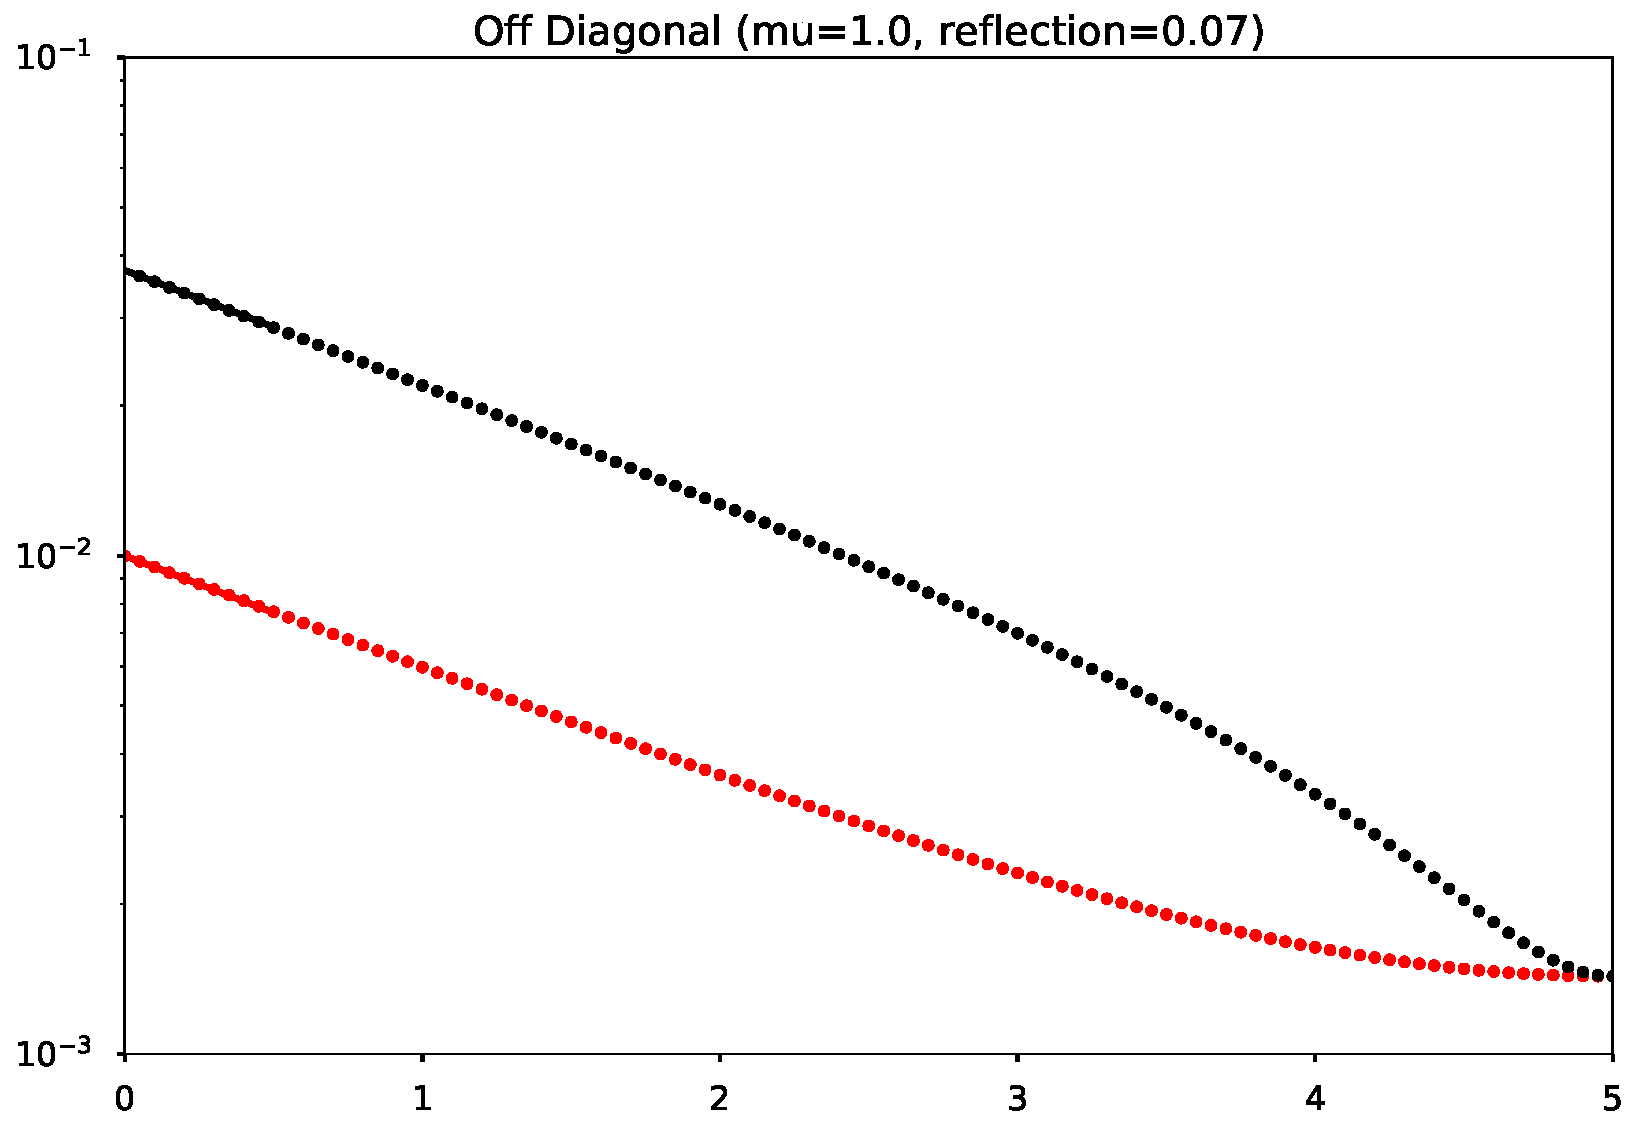
\includegraphics[width=\textwidth]{assets/halo-mu-1-reflection-0p07}
      \end{figure}
      % }

   % \only<2>{
   %    \begin{figure}
   %       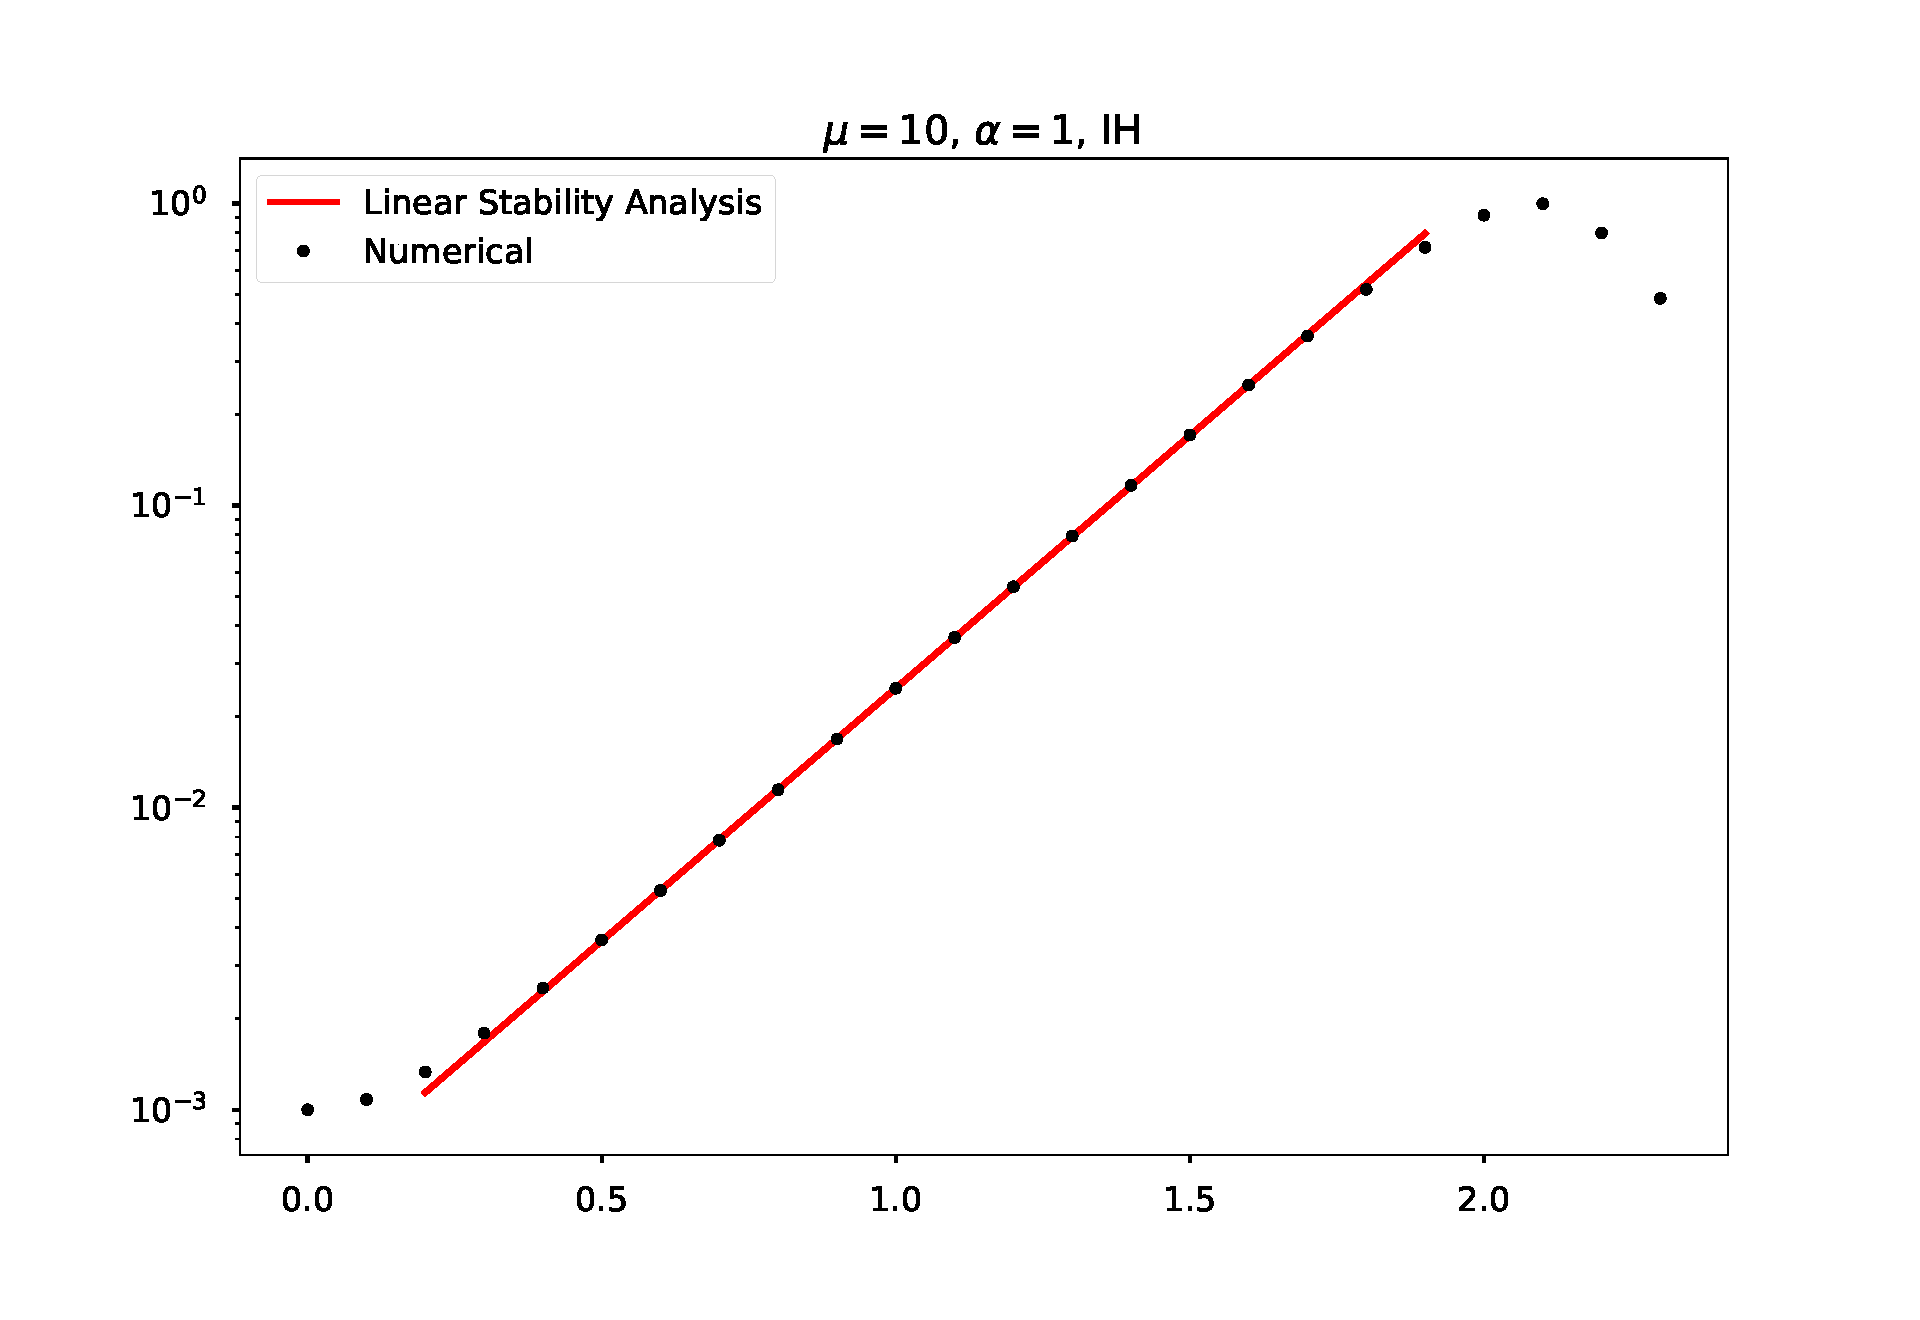
\includegraphics[width=\textwidth]{assets/halo-mu-4-compare-bipolar}
   %    \end{figure}
   % }

\end{tcolorbox}



\end{frame}
